\section{Ausführung}

\subsection{Einführung}

\begin{frame}[c]{Problem: Ausführung}
    \large
    \begin{aquote}{Chris Sacca (Shark Tank)}
        Ideas are cheap. It's all about execution.
    \end{aquote}
    \pnote{Gibt grundsätzlich Zwei Perspektiven zur Ausführung}
\end{frame}


\begin{frame}[c]{Perspektive: Kurzfristig}
    \large
    \begin{itemize}
        \item Pomodoro
        \item Time-Blocking
        \item Arbeitszyklen
        \item Kaffee/Koffein
        \item Co-Working-Räume
        \item \enquote{Einfach machen}
    \end{itemize}
\end{frame}


\addtocounter{framenumber}{1}
\begin{frame}[standout]
    \Large
    Jetzt: Langfristig
\end{frame}

% > Ideas are cheap. It’s all about execution. - Chris Sacca (Shark Tank)
%
% While we already defined the first three next action items for each of your
% goals, they should be done the day after tomorrow. What then?
%
% There are two parts to execution, and they answer different timeframes to the
% questions ‘what do I do next?’.
%
% First is how to execute in the moment: While just sitting down and working on
% it is pretty effective, there are some techniques you might at least want to
% try, which could spice things up a bit. But just working and working and
% working on something is not guaranteed to work out. Being busy is absolutely
% not the same as being effective. Keeping the ships nose pointed east is fine,
% but you need to make sure that it’s moving as well.
%
% Second is the bigger-picture planning and execution. This includes taking a
% look at all the projects you want to work on, the tasks you have left, your
% progress and your current results, to determine if you’re going the right
% way. To determine that the ship is actually moving forward while pointed
% east. We’re primarily going to take a look at that one.
%
% We will take a look as to why execution tends to fail in the first place, to
% understand why an execution system is a decent approach to addressing these
% issues properly.


\subsection{Häufige Probleme}

\begin{frame}[c]{Häufige Probleme}
    % \large
    \footnotesize
    \begin{itemize}[<+(1)->]
        \item Aversion: Es ist unangenehm, über das Ziel oder die Ausführungspläne nachzudenken (Stress, Selbstschuld, Angst)
        % \item Aversion: When thinking about our goals or execution plans, we experience some form of discomfort (stress, guilt, dread)
        \item Ablenkung: Wir suchen andere angenehme Dinge, um uns abzulenken und prokrastinieren
        % \item Distraction: Instead of doing the hard work, we procrastinate and distract ourselves with urgent or pleasurable things instead
        % \item Zu wenig Motivation: Unser Ziel und unsere Pläne geben uns nicht mehr genug Energie
        % \item Limited motivation: Somehow our goal and our plans don’t give us energy any more
        \item Zu wenig Zeit: Wir sind mit etwas anderem beschäftigt
        % \item Limited time: It’s easy to be busy in the moment and focus on other things instead
        \item Zu wenig Energie: Wir sind zu müde, nach der Arbeit noch etwas weiteres zu tun
        % \item Limited energy: We are too tired to work on something else after a long day at work
        \item Zu wenig Aufmerksamkeit: Es ist nicht wirklich klar, was der nächste Schritt ist
        % \item Limited attention: It’s not even clear what we want to do, since it’s hard to keep track of everything
        \item Zu wenig Verantwortung: Es ist selten, dass jemand von uns erwartet, dass es fertig wird
        % \item Limited accountability: We rarely have someone else holding us accountable, resulting in conscious and unconscious guilt to increase accountability.
        \item Zu wenig Selbstvertrauen: Niedrige Selbstwirksamkeit ist eine sich selbst erfüllende Prophezeiung; Wir erwarten nicht, das Projekt abzuschließen
        % \item Limited self trust: A low self-efficacy self-fulfilling prophecy; We don’t think we will ultimately follow through, so we won’t
    \end{itemize}
\end{frame}


\begin{frame}[c]
    \begin{block}{Aufgabe: Grund für Misserfolg finden}
        Finde heraus, weswegen dein letztes größeres Projekt gescheitert ist,
        und was du diesmal anders machen könntest.
    \end{block}
    \pnote{5min}
\end{frame}


\begin{frame}[c]{Optional: Murphyjitsu}
    \large
    \begin{enumerate}[<+(1)->]
        \item Mache einen Plan.
        \item Stell dir vor, der Plan ist gescheitert.
        \item Wenn du überrascht von der Vorstellung bist, bist du fertig.
        \item Andernfalls, simuliere den wahrscheinlichsten Fehlermodus. Unternehme etwas dagegen. Wiederhole ab Schritt 2.
    \end{enumerate}
    \pause
    \tiny
    Mehr Informationen: \url{https://www.lesswrong.com/posts/N47M3JiHveHfwdbFg/hammertime-day-10-murphyjitsu}
\end{frame}


\begin{frame}[c]
    \begin{block}{Aufgabe: Murphyjitsu}
        Finde heraus, weswegen deine Ziele scheitern könnten, und unternehme
        etwas gegen wahrscheinliche Blockaden.
    \end{block}
    \pnote{Zeit: 20min}
\end{frame}


% Failing Execution (5min)
% Execution tends to regularly fail, and there is a number of reasons why.
% Taking some time to think about root causes, you might end up with a list
% similar to this:
%
% - Aversion: When thinking about our goals or execution plans, we experience some form of discomfort (stress, guilt, dread)
% - Distraction: Instead of doing the hard work, we procrastinate and distract ourselves with urgent or pleasurable things instead
% - Limited motivation: Somehow our goal and our plans don’t give us energy any more
% - Limited time: It’s easy to be busy in the moment and focus on other things instead
% - Limited energy: We are too tired to work on something else after a long day at work
% - Limited attention: It’s not even clear what we want to do, since it’s hard to keep track of everything
% - Limited accountability: We rarely have someone else holding us accountable, resulting in conscious and unconscious guilt to increase accountability.
% - Limited self trust: A low self-efficacy self-fulfilling prophecy; We don’t think we will ultimately follow through, so we won’t
%
% In fact, it might not be just one, it might be multiple reasons at once. And
% sometimes, that’s fine - as long as you don’t beat yourself up over it.
%
% There are ways to improve in-the-moment effectiveness, but they are band-aid
% at best and don’t help if you can’t get started in the first place. Execution
% systems go for multiple of these potential failure modes at once, helping us
% tremendously in achieving our goals.
%
% Figure out the main reasons why your last project or goal was unsuccessful,
% and what you would change next time.


\subsection{Verantwortungspartner}

% Forschung: 149/267 Teilnehmer
% Zufällig gruppe zugewiesen
% - gruppe 1 hat sich über die Ziele gedanken gemacht
%   rate that goal on the following dimensions: Difficulty, Importance, the
%   extent to which they had the Skills & Resources to accomplish the goal,
%   their Commitment and Motivation to the goal, whether or not they had
%   Pursued this goal before and if so their Prior Success.
% jede gruppe hat auch das getan, was die gruppe davor getan hat
% - Participants in Groups 2-5 were asked to write (type into the online survey)
% their goals and then to rate their goals on the same dimensions.
% - Group 3 was also asked to formulate action commitments.
% - Group 4 was asked to formulate action commitments and send their goals and
% action commitments to a supportive friend.
% - Group 5 was asked to formulate action commitments and send their goals,
% action commitments and weekly progress reports to a supportive friend.

\begin{frame}[c]{Fortschrittsberichte}
    \small
    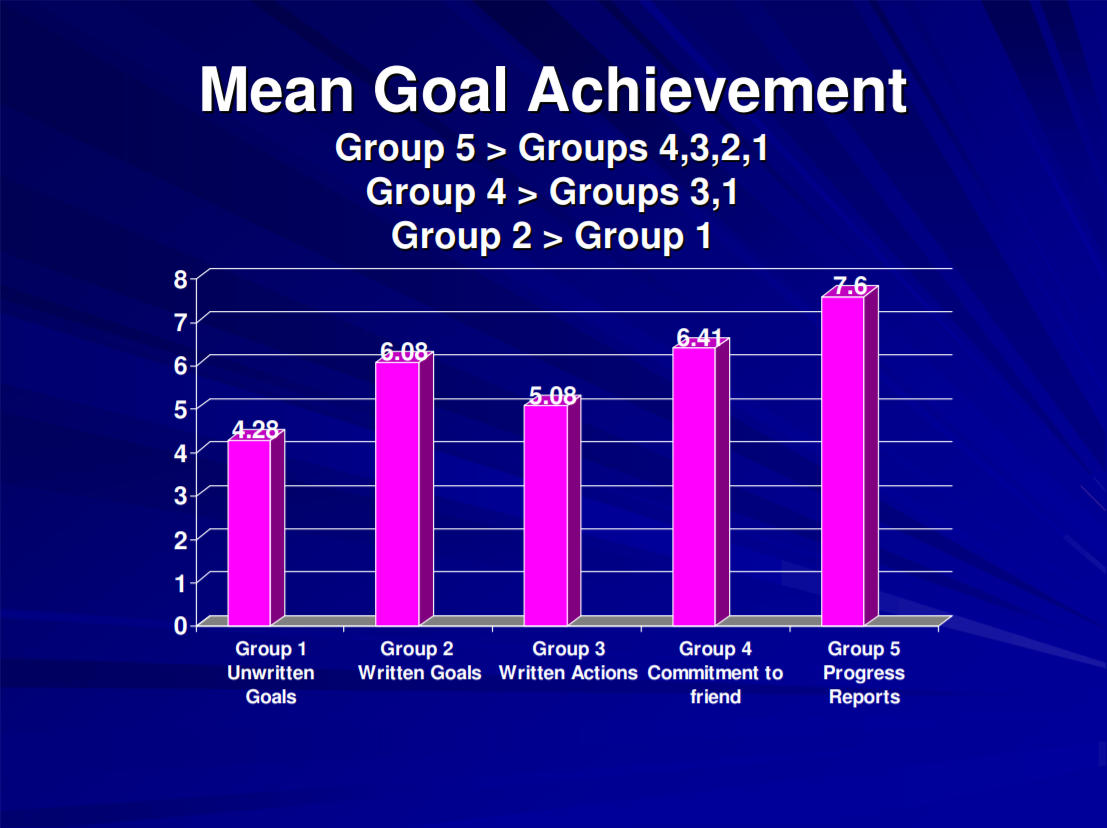
\includegraphics[height=0.8\textheight]{goal_achievement_all} \\
    Regelmäßige Fortschrittsberichte haben den höchsten Erfolg \cite{better-goals-2}.
    \pnote{Jede Gruppe auch immer das von den vorigen}
    \pnote{Gruppe 1: Gedanken gemacht über Schwere, Wichtigkeit, Fähigkeiten, Motivation, etc}
    \pnote{Gruppe 2: Aufschreiben}
    \pnote{Gruppe 3: 'Formulate Action Commitments'}
    \pnote{Gruppe 4: Send goals and action commitments to friend}
    \pnote{Gruppe 5: Send weekly progress reports to supportive friend}
\end{frame}


\begin{frame}[c]{Interaktion mit Verantwortungspartner}
    \begin{enumerate}[<+(1)->]
        \item Finde jemanden, mit dem du dich regelmäßig verabreden kannst
        \item Berichte von deinem Fortschritt seit dem letzten Treffen
        \item Gebe an, was deine nächsten Schritte sind, und was du bis zum nächsten Treffen erreichen möchtest
        \item Vereinbare den nächsten Termin
        \item Beim nächsten Treffen: Starte ab dem zweiten Schritt
    \end{enumerate}
    \pnote{Wichtig: Nicht Ziele 'Bewerten' lassen, gibt Studien, dass Erfolg reduziert}
\end{frame}


\begin{frame}[c]
    \begin{block}{Aufgabe: Finde einen Verantwortungspartner}
        Finde jemanden, mit dem du dich regelmäßig über deinen
        Fortschritt austauschen kannst, und vereinbare den ersten Termin.
    \end{block}
    \pnote{Zeit: 10min}
\end{frame}

% Accountability Partners (10min)
% One very simple way that will help you to get started and to keep doing it,
% is to have someone hold you accountable for it. In fact, it is a very simple
% execution system and will help a lot with the common failure modes.
%
% It mostly does not matter who will hold you accountable, but a friend who
% needs someone to hold them accountable for something themselves is ideal.
% Just schedule a meeting or call every week, month, or other timeframe you are
% comfortable with, and you’re good to go.
%
% The goal is that you state your goals and the progress you want to make each
% meeting and get asked about the progress you actually achieved prior to
% planning your progress the next meeting. That’s it. Repeat.
%
% Here are the steps again:
%
% - Find a friend to hold you accountable and schedule regular calls or meetings
% - Report progress and current challenges on your goal(s)
% - State your next steps and what you want to achieve until next time (Lead measures!)
% - Schedule the next call/meeting before hanging up/separating
% - Repeat from Step 2 at the next call/meeting
%
% Obviously you shouldn’t talk the entire time. Intersperse your meeting with
% listening to the progress and next steps of your friend. I’m doing my monthly
% planning similarly with a friend, and it helped me tremendously to stay
% focused and to achieve more. In our experience, talking about
% non-goal-related topics in the first few minutes is a good and comfortable
% way to start.
%
% Find yourself an accountability partner and schedule the first meeting.
%
% You might want to take a look at Execution Systems before actually doing so.
% It explains a similar system that is synergistic with Accountability
% Partners, if implemented right.





% \subsection{Selbstmanagementsysteme}


% Setting up an Execution System (30min)
% Accountability Partners is in itself a basic Execution System, and works best
% when implemented with a second Execution System over a different timeframe.
%
% Fundamentally, every execution system has these four parts, weighed as required:
%
% Review: Taking a look at the progress that happened, evaluating taken approaches
% Retrospective: Taking a look at the current process, making adjustments for parts that are not working as well as they should
% Planning: Planning milestones and tasks for the next timeframe until Review, clarifying when they are done
% Execution: Actually working on the collected Tasks, in a way to make progress on them.
% Another very important parameter is your cycle frequency, or how long it takes for a full cycle in your Execution System. We’ll take a look at each of these parts in detail, before we discuss how to implement it.
%
% Review
% A regular review is the single most important part in an execution system. It
% enables both planning and execution to build on the most recent insights of
% how things stand.
%
% The goal is to get a bigger-picture perspective about the goals you are
% working on. The most important part is reviewing what was planned and what
% was achieved, and just generally taking inventory of made progress. If you
% haven’t marked some tasks as done yet, now is the time to bring your notes up
% to date.
%
% A big focus is how you approach the problems you encounter and how well your
% approaches are working. If they’re not working well, you adjust them during
% ‘Retrospective’, to do better next cycle.
%
% When collecting decent Lead/Lag metrics, plotting them can be really useful
% in noticing outliers and general trends. It is also motivating to see the
% progress that has been made, making it easier to keep going.
%
% Retrospective
% This is the phase to make changes to your execution system and how to use it,
% to adapt it to your needs. Beware of many changes at once, since a single
% change can modify the nature of Execution Systems tremendously. It’s not
% necessary to make changes all the time, but if there’s something bugging you,
% figure out a way to improve it. Even small changes can help you substantially
% - especially in the long run.
%
% This is also the time to figure out solutions for obstacles preventing you to
% execute during ‘Execution’ - e.g. getting a ‘Do not disturb’-sign to tell
% your flatmates when you prefer not to get interrupted.
%
% If you noticed that a Lead or Lag measure does not fit for the goal or
% milestone, now is the time to make adjustments.
%
% Planning
% This is more or less a ‘mini’-planning section, with the core focus being to
% ensure you have at least one if not multiple next actions for each goal and
% project.
%
% After reviewing the progress and status for all of your projects and goals,
% you might need to plan or adapt the next steps for each. It might not be
% necessary, but more often than not I notice a missing task, clarify
% descriptions or reorganize priorities.
%
% Execution
% When actually working on tasks, it can be helpful to try one of the following
% productivity helpers:
%
% Pomodoro
% Work Cycles
% Co-Working Spaces
% A ‘Pomodoro’ is a 30-min interval with 25min work-time and a break of 5min.
% Work Cycles are similar, with 30min work time interspersed with 10min breaks,
% in which you do a bit of work-related planning and reviewing.
%
% Co-Working spaces such as libraries are great, many have found themselves to
% be much more productive there. It’s harder to let yourself slack off, and
% easier to stay productive, with or without pomodoro. A virtual co-working
% space such as the LessWrong study hall can have the same effects.
%
% However, it’s all about actually getting your next action items done, and
% making progress on your goals, projects and milestones. So feel free to use
% whatever method best works for you.
%
% Timeframe
% The timeframe you plan for is an important factor. It can be anything you are
% comfortable with, but I would recommend a one-week-cycle as a basis with a
% complementary one-month-cycle of Accountability Partners. But a weekly cycle
% is essential to enable continuous execution of your goals.
%
% Putting Everything Together
% Your execution system should enable you to easily figure out what you both
% want and need to do in the moment. New tasks get added during the weekly
% review/planning session as well as when something comes up during the week.
%
% The core parts to enable that is the weekly review - it is normal to forget
% details during the week. I tend to have both completed tasks not yet marked
% as done as well as new open tasks not yet included, but maybe written down
% somewhere else. The weekly review is the time to synchronize the execution
% system to what happened in the real world.
%
% As long as your execution system is (mostly) current when taking a look at it
% during the week, you are able to get the open tasks that require your
% attention now.
\fpause
